\chapter{\MakeUppercase{Results and Discussion}}

\section{Introduction}
\paragraph{}
This chapter presents the experimental outcomes of the fairness-aware credit scoring pipeline and discusses their implications in practical decision-making. The focus is not limited to identifying the highest-performing model, but rather on determining the most suitable model–fairness configuration based on dataset characteristics and institutional risk appetite.

The chapter includes empirical results, statistical analysis, cross-dataset observations, and a practical decision-making framework for real-world adoption.

\section{Experimental Result Summary}
\paragraph{}
The experiment evaluated three datasets (Australian, German, and GMSC), six model families, and five fairness levels (0.0, 0.25, 0.5, 0.75, 1.0), resulting in a total of 90 configurations.

The following output artifacts were generated:
\begin{itemize}
    \item results.csv
    \item subgroup\_metrics.csv
    \item paired\_tests.csv
    \item Visualization figures in output folders
\end{itemize}

\section{Dataset-Wise Findings}

\subsection{Australian Dataset}
\paragraph{}
Key observations:
\begin{itemize}
    \item Best baseline: XGBoost @ fairness level 0.0 (Accuracy = 0.8696, DP = 0.0407)
    \item Best overall accuracy: XGBoost @ 0.5 (Accuracy = 0.8768, DP = 0.0719)
    \item Best fairness: Random Forest @ 0.0 (DP = 0.0029, Accuracy = 0.8116)
    \item Balanced point: Gradient Boosting @ 0.0 (Accuracy = 0.8261, DP = 0.0218)
\end{itemize}

The dataset exhibits a clear fairness–accuracy trade-off, making it suitable for policy-driven selection.

\begin{figure}[h]
\centering

\includegraphics[width=0.9\textwidth]{images/australian_tradeoff.png}
\caption{Australian Fairness-Performance Trade-off}
\end{figure}

\begin{figure}[h]
\centering

\includegraphics[width=0.9\textwidth]{images/australian_dp_diff.png}
\caption{Australian DP Difference vs Fairness Level}
\end{figure}

\subsection{German Dataset}
\paragraph{}
Key observations:
\begin{itemize}
    \item Best baseline: XGBoost @ 0.0 (Accuracy = 0.7600, DP = 0.0952)
    \item Best accuracy: Gradient Boosting @ 0.5 (Accuracy = 0.7800, DP = 0.0286)
    \item Best fairness: XGBoost @ 0.75 (DP = 0.0000, Accuracy = 0.7200)
    \item Balanced point: Gradient Boosting @ 0.25 (Accuracy = 0.7600, DP = 0.0048)
\end{itemize}

The dataset responds effectively to fairness tuning, especially in boosting-based models.

\begin{figure}[h]
\centering

\includegraphics[width=0.9\textwidth]{images/german_tradeoff.png}
\caption{German Fairness-Performance Trade-off}
\end{figure}

\begin{figure}[h]
\centering

\includegraphics[width=0.9\textwidth]{images/german_dp_diff.png}
\caption{German DP Difference vs Fairness Level}
\end{figure}

\subsection{GMSC Dataset}
\paragraph{}
Key observations:
\begin{itemize}
    \item Best baseline and best accuracy: XGBoost @ 0.0 (Accuracy = 0.9383, DP = 0.0243)
    \item Best fairness and balanced point: Logistic Regression @ 0.25 (Accuracy = 0.9340, DP = 0.0085)
\end{itemize}

This dataset shows that fairness improvements can be achieved with minimal loss in predictive performance.

\begin{figure}[h]
\centering
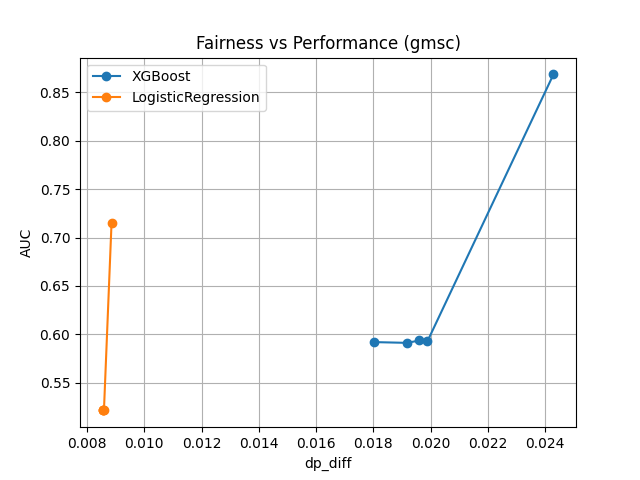
\includegraphics[width=0.9\textwidth]{images/gmsc_tradeoff.png}
\caption{GMSC Fairness-Performance Trade-off}
\end{figure}

\begin{figure}[h]
\centering
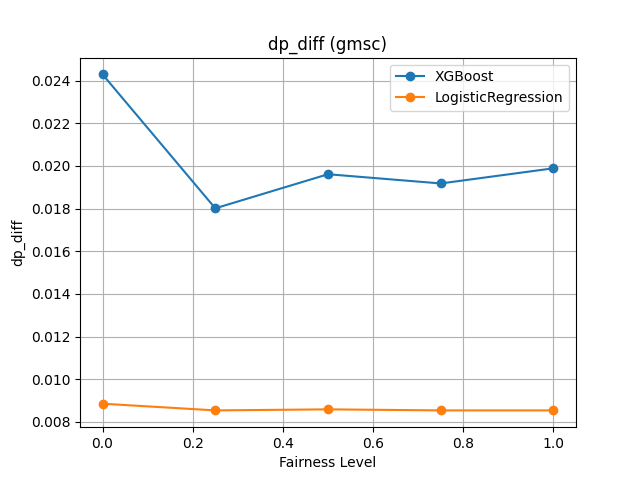
\includegraphics[width=0.9\textwidth]{images/gmsc_dp_diff.png}
\caption{GMSC DP Difference vs Fairness Level}
\end{figure}

\section{Statistical Reliability Discussion}
\paragraph{}
Paired t-tests were conducted to evaluate whether observed performance differences are statistically significant.

Observed significant comparisons (p < 0.05):
\begin{itemize}
    \item Australian: $\sim$12.5\%
    \item German: $\sim$12.5\%
    \item GMSC: $\sim$16.7\%
\end{itemize}

These results indicate that not all observed differences are statistically strong, highlighting the need for validation before decision-making.

\begin{figure}[h]
\centering
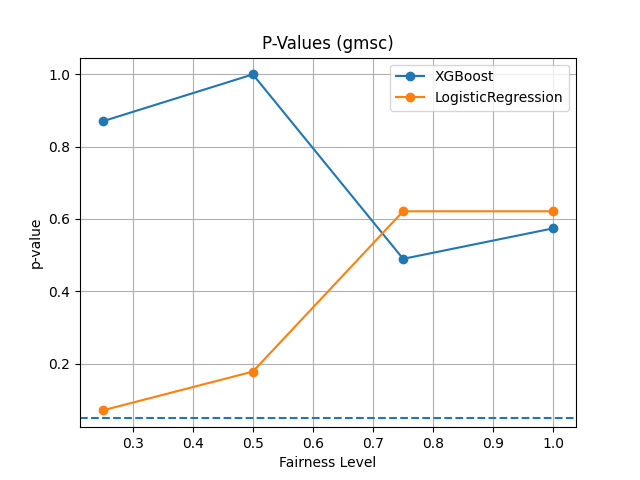
\includegraphics[width=0.9\textwidth]{images/gmsc_pvalues.png}
\caption{GMSC p-value Trend Across Fairness Levels}
\end{figure}

\begin{figure}[h]
\centering
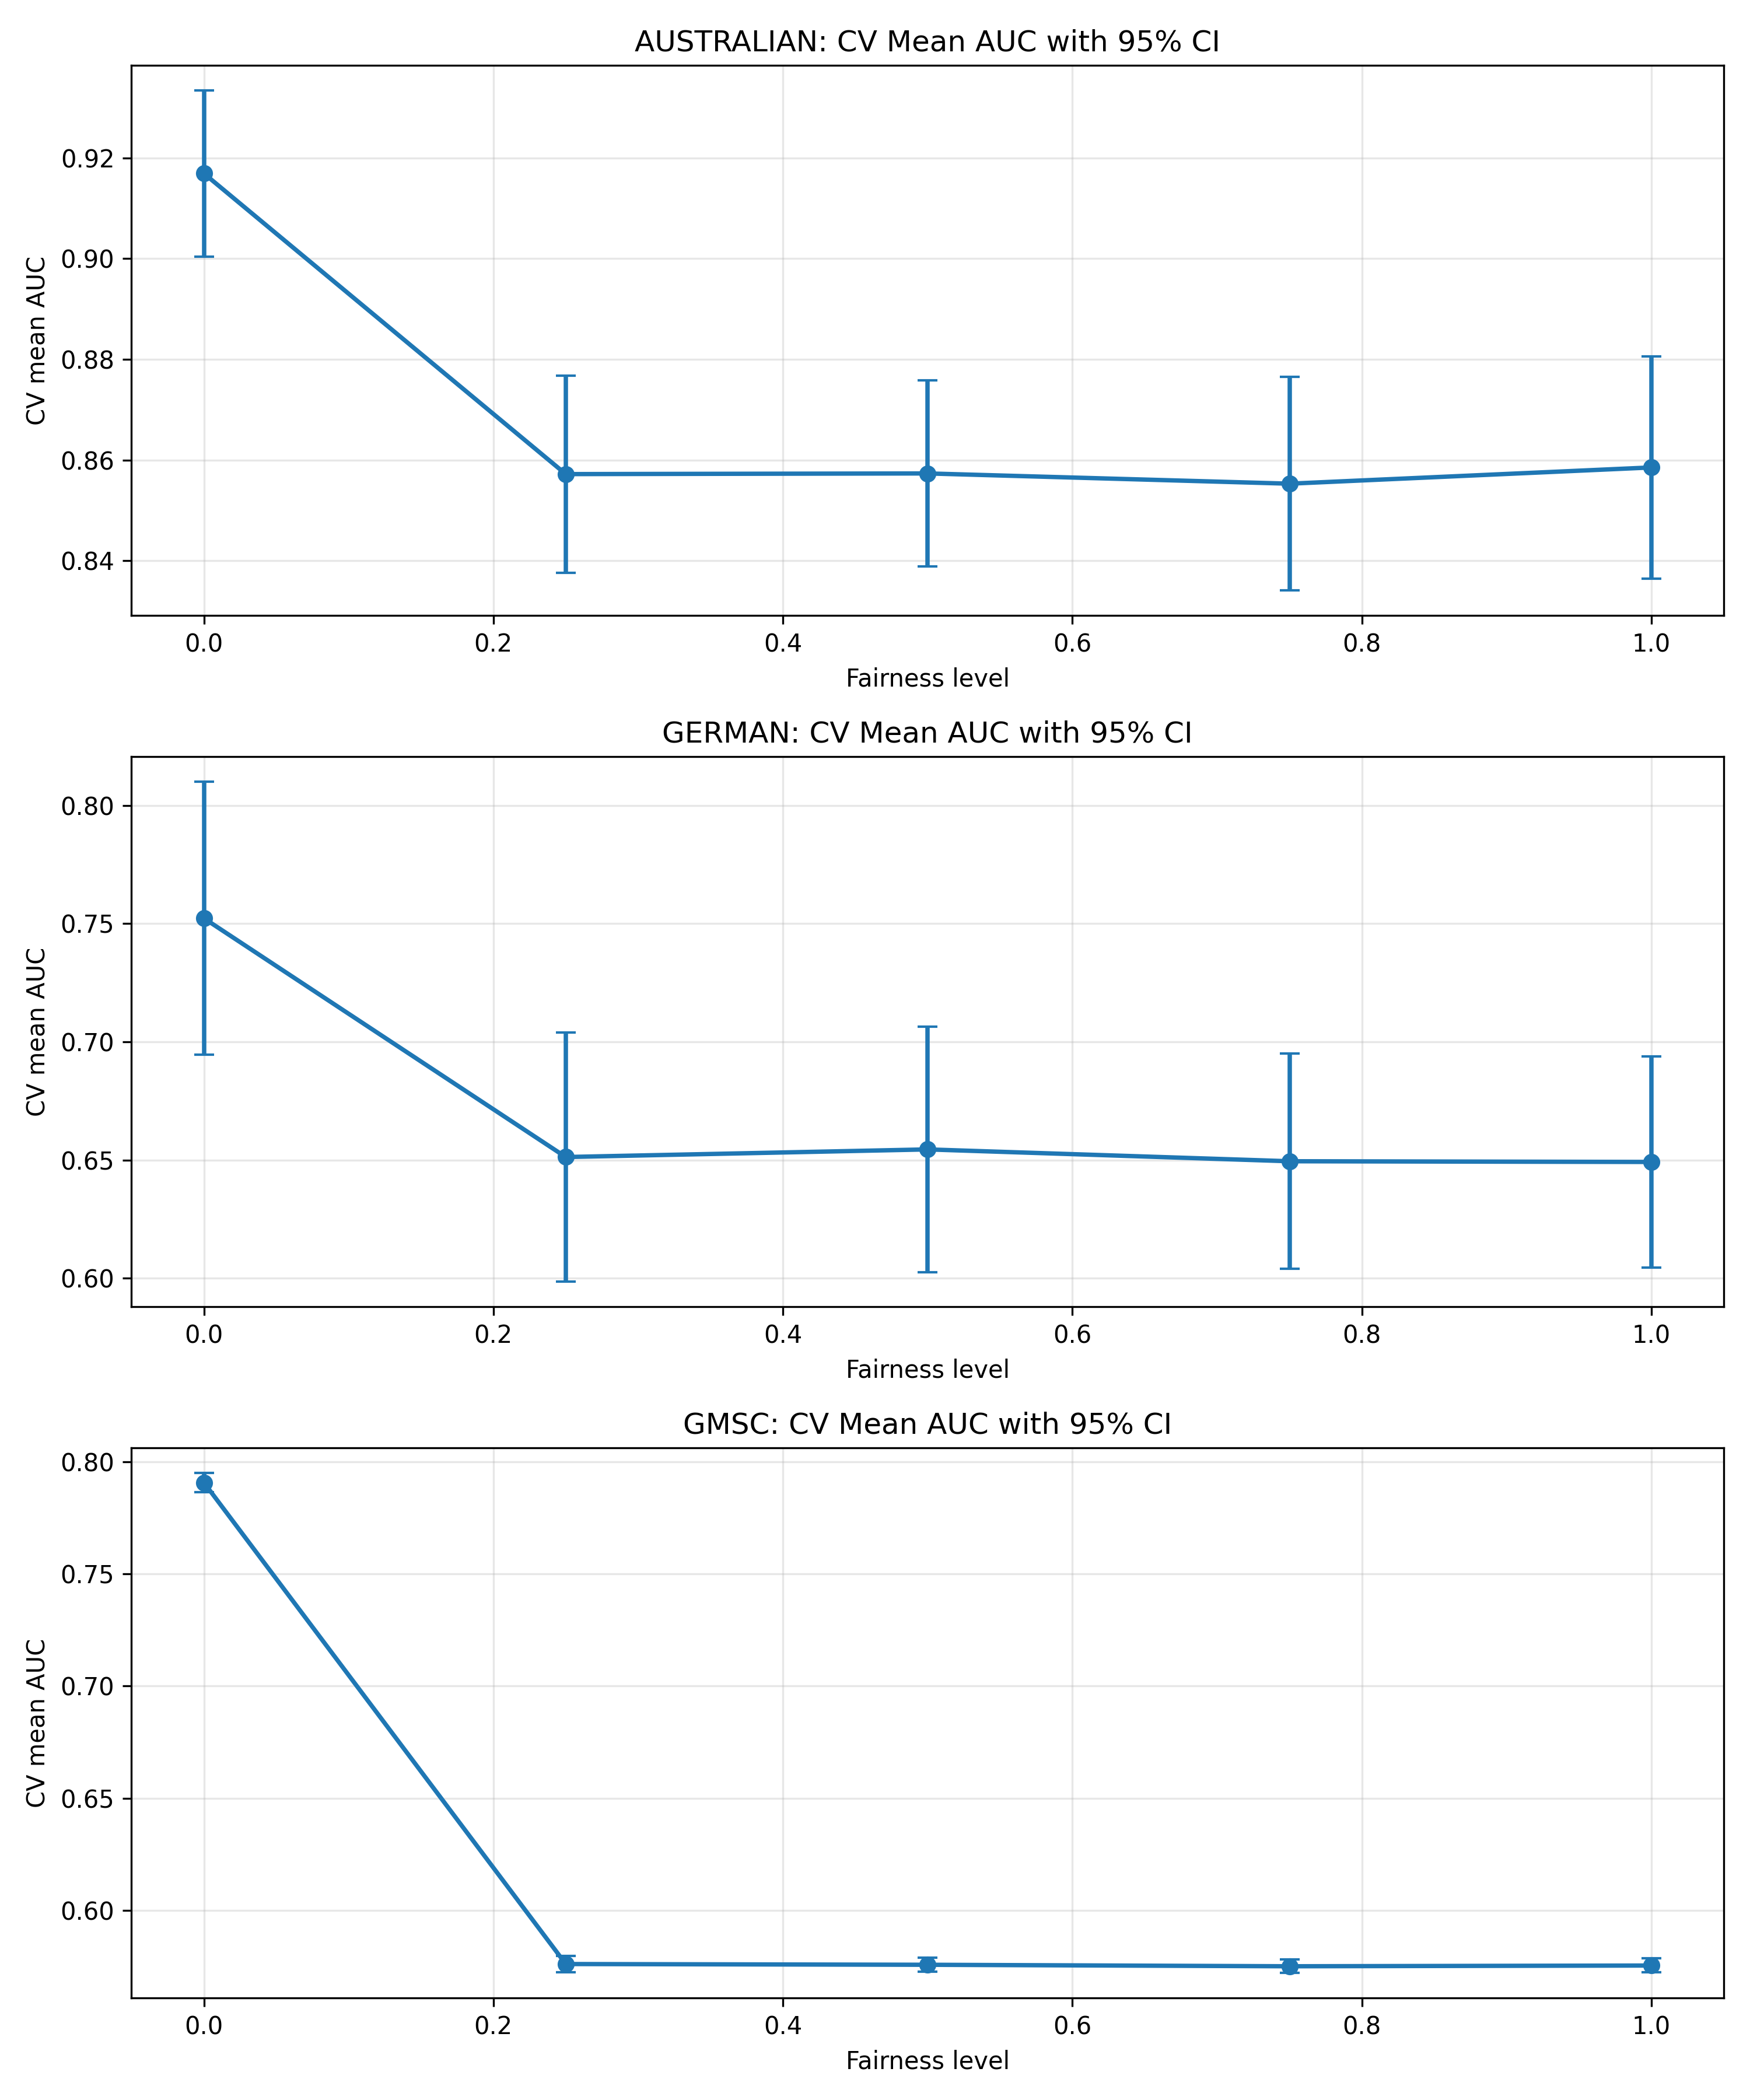
\includegraphics[width=0.9\textwidth]{images/figure_ci_auc_95.png}
\caption{CV Mean AUC with 95\% Confidence Intervals}
\end{figure}

\section{Cross-Dataset Behavioral Patterns}
\paragraph{}
The following consistent patterns were observed:
\begin{itemize}
    \item No single model is optimal for both fairness and accuracy
    \item Fairness impact is dataset-dependent
    \item Optimal solutions lie on the trade-off frontier
    \item Statistical and subgroup validation are necessary
\end{itemize}

\section{Proposed Practical Framework for Banks}

\subsection{Core Idea}
\paragraph{}
The framework converts experimental results into a structured decision process involving dataset classification, model selection, operating point choice, and validation.

\subsection{Dataset Classification}
\paragraph{}
Three diagnostic metrics are used:

\begin{itemize}
    \item Group Balance Ratio (GBR)
    \item Absolute Base Rate Gap (ABG)
    \item Relative Base Rate Ratio (RBR)
\end{itemize}

\begin{table}[h]
\centering
\caption{Metric Scoring Table}
\renewcommand{\arraystretch}{1.3}
\begin{tabular}{|c|c|c|c|}
\hline
Metric & Low & Medium & High \\ \hline
GBR & $\leq$1.5 & 1.5--2.5 & $>$2.5 \\ \hline
ABG & $\leq$0.03 & 0.03--0.07 & $>$0.07 \\ \hline
RBR & $\leq$1.2 & 1.2--1.6 & $>$1.6 \\ \hline
\end{tabular}
\end{table}

\paragraph{}
Composite score:
\[
\text{SkewScore} = GBR_{pts} + ABG_{pts} + 2 \times RBR_{pts}
\]

\section{Model Shortlisting}
\paragraph{}
\begin{table}[h]
\centering
\caption{Model Selection by Dataset Type}
\renewcommand{\arraystretch}{1.3}
\begin{tabular}{|c|c|c|c|}
\hline
Dataset Type & Primary & Secondary & Caution \\ \hline
Balanced & XGBoost, RF, GB & Logistic Regression & None \\ \hline
Moderate & GB, XGBoost, EBM & Logistic Regression & Unstable curves \\ \hline
High Skew & EBM, GB, LR & XGBoost & Avoid unstable trees \\ \hline
\end{tabular}
\end{table}

\section{Policy-Based Selection}
\paragraph{}
Operating point selection is based on fairness–accuracy trade-off graphs.

\begin{table}[h]
\centering
\caption{Policy Thresholds}
\renewcommand{\arraystretch}{1.3}
\begin{tabular}{|c|c|c|c|}
\hline
Mode & Accuracy Floor & DP Cap & EO Cap \\ \hline
Profit-first & $\geq$98\% & $\leq$0.08 & $\leq$0.12 \\ \hline
Balanced & $\geq$95\% & $\leq$0.03 & $\leq$0.08 \\ \hline
Fairness-critical & $\geq$90\% & $\leq$0.015 & $\leq$0.05 \\ \hline
\end{tabular}
\end{table}

\begin{figure}[h]
\centering
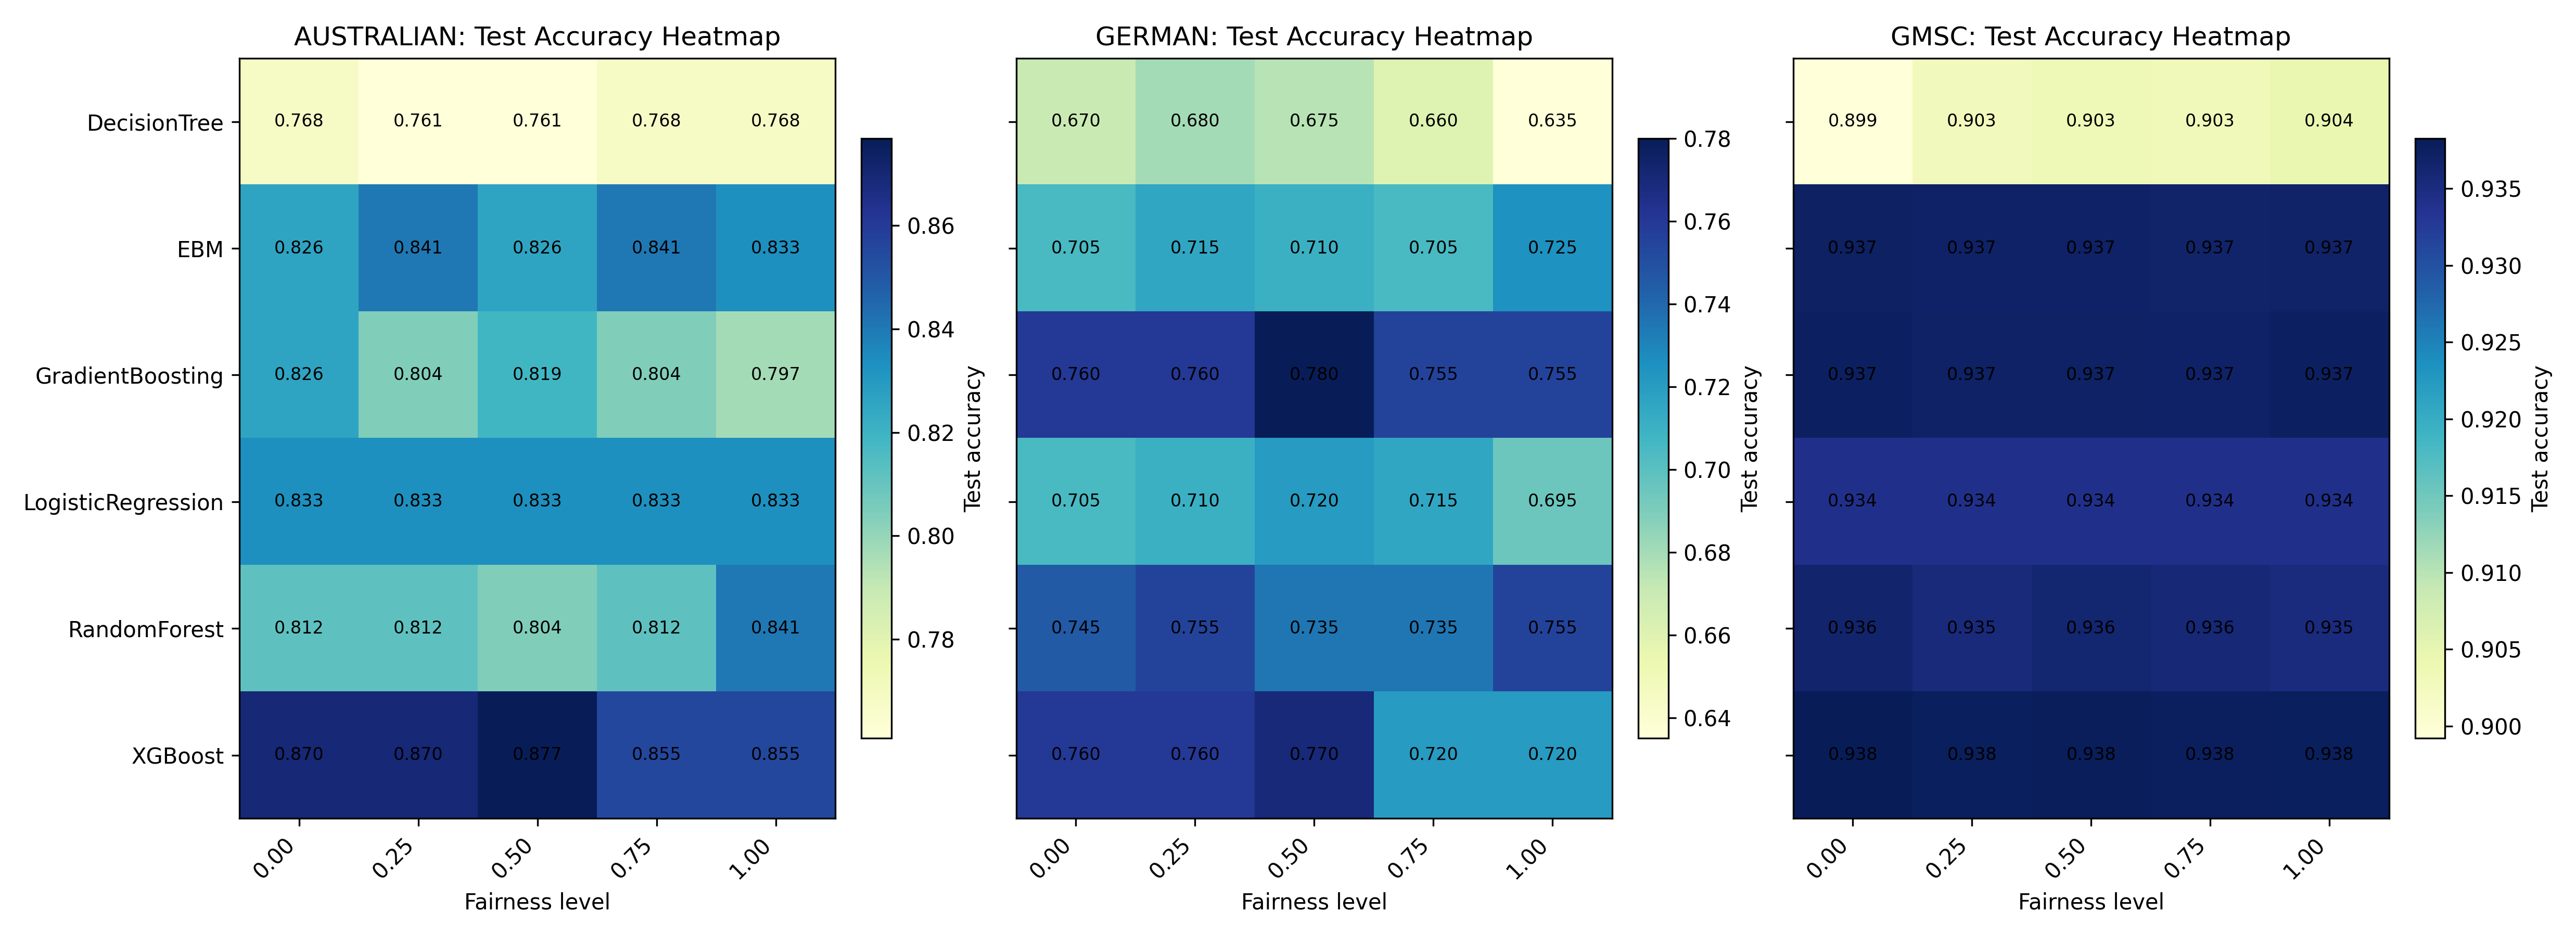
\includegraphics[width=0.9\textwidth]{images/figure_accuracy_heatmap.png}
\caption{Accuracy Heatmap by Model and Fairness Level}
\end{figure}

\section{Validation Before Deployment}
\paragraph{}
Selected configurations must satisfy:
\begin{itemize}
    \item Statistical significance
    \item Curve stability
    \item Acceptable subgroup behavior
    \item Reproducibility
\end{itemize}

\section{Operational Pipeline for Banks}
\paragraph{}
\begin{table}[h]
\centering
\caption{Operational Decision Pipeline}
\renewcommand{\arraystretch}{1.3}
\begin{tabular}{|c|c|c|c|}
\hline
Stage & Question & Action & Output \\ \hline
Diagnose & Data type? & Compute metrics & Dataset type \\ \hline
Shortlist & Model choice? & Use table & Candidates \\ \hline
Select & Trade-off? & Choose point & Final config \\ \hline
Validate & Reliable? & Statistical checks & Approve/reselect \\ \hline
\end{tabular}
\end{table}

\section{Practical Implications}
\paragraph{}
Fairness should be treated as a policy-driven operating point rather than a static model choice. Structured selection improves transparency, compliance, and interpretability in financial decision-making.

\section{Chapter Summary}
\paragraph{}
This chapter demonstrated that fairness-aware model selection requires a structured approach involving dataset diagnosis, model selection, policy-based trade-off choice, and statistical validation. The proposed framework provides a practical and reproducible pathway for deploying fair and effective credit scoring systems.